% Compilar usando LuaLaTeX.

\documentclass{book}

% Configuraciones:

% O comando abaixo pode ser necessário em documentos que usam versões antigas do pacote "fontspec". Se for começar um novo documento, deixe esse linha comentada e use caracteres Unicode.
% \usepackage[utf8]{luainputenc}


% Licencia CC
\usepackage[
    type={CC},
    modifier={by-sa},
    version={3.0},
    lang={sp},
]{doclicense}
% Tamanho do papel e das margens: 
\usepackage{rotating}
\usepackage[paperheight=230mm,paperwidth=160mm,inner=20mm,outer=14mm,top=24.5mm,bottom=21mm,pdftex]{geometry}

% Suporte a idiomas:

\usepackage[greek,brazilian,spanish]{babel}

% Para usar as variáveis \theauthor, \thetitle e \thedate (autor, título e data).

\usepackage{titling}

% Título de capítulo elegante:

\usepackage[Lenny]{fncychap}

% Pacote para estilo elegante:

\usepackage{fancyhdr}

% Definição de novas cores:

\usepackage{xcolor}

\definecolor{verde}{rgb}{0.2, 0.50, 0.25}
\definecolor{verde_UnB}{cmyk}{1,0,1,0.4}
\definecolor{cinza_UnB}{rgb}{0.6,0.6,0.6} % https://www.ginifab.com/feeds/pms/color_picker_from_image.php


% Para mudar cor de títulos (https://tex.stackexchange.com/a/75670/91816):

\usepackage{sectsty}

\chapterfont{\color{verde_UnB}}  % sets colour of chapters
\sectionfont{\color{verde_UnB}}  % sets colour of sections

% Pacote para definir fonte de qualquer tamanho:

\usepackage{fix-cm}

%% Pacote para correta separação silábica de palavras com hífen;
%% hífens devem ser escritos como \Hyphdash ou \-/ (se opção shortcuts estiver ativa)
%% no texto; por exemplo cana\-/de\-/açúcar seria separada como
%% cana-de- numa linha e -açúcar na linha seguinte
%% repetindo o hífen (um hífen é da separação e outro é da palavra):

\usepackage[shortcuts]{extdash}

%% Definindo espacamento:

\usepackage{setspace} 
\singlespacing

%% Enumerar itens:

\usepackage{enumitem}

%% Pacote para criar caixas:

\usepackage{pbox} %  que limitam a largura de textos em células,
%\usepackage{minibox} % que têm largura arbitrária.

%% Definição das dimensões do texto:

%\setlength{\textwidth}{16cm}
%\setlength{\textheight}{22cm}
%\setlength{\headheight}{1cm}
%\setlength{\footheight}{1cm}

\usepackage[title,titletoc]{appendix}

%% Passando títulos para o português:

\renewcommand{\chaptername}{Capítulo}
\renewcommand{\bibname}{Referencias}
\renewcommand{\appendixname}{Anexo}
\renewcommand{\indexname}{Índice}
\renewcommand{\contentsname}{\bf\color{verde_UnB}Contenidos}
\renewcommand{\tablename}{Tabla}
\renewcommand{\figurename}{\bf Fig.}
\renewcommand{\sin}{sen}
\def\listoffiguresname{Lista de Figuras}
\def\listoftablesname{Lista de Tablas}

%% Definindo estilo de pagina:

\pagestyle{fancy}

% PACOTES DE TABELAS:

%% Espaçamento de tabelas ajustado:

\usepackage{booktabs}

%% Pacotes de linhas e colunas multiplas:

\usepackage{multirow}
\usepackage{multicol}

%% Pacotes de tabela e tabulação:

%%% Tabela com caixas centralizada:

\usepackage{array}
\newcolumntype{P}[1]{>{\centering\arraybackslash}p{#1}}

%%% Tabela em múltiplas páginas:

\usepackage{longtable}

%%% Tabela colorida:

\usepackage{tabu}
\usepackage{colortbl}

%%% Mudando cor das linhas de todas as tabelas:

\makeatletter
\renewenvironment{table}
     {\@float{table}\taburulecolor{verde_UnB}\arrayrulecolor{verde_UnB}}
     {\end@float}
\makeatother

%%% Tabela com linhas pontilhadas:

\usepackage{arydshln}

% PACOTES MATEMÁTICOS:

%% Pacote para não-itálico em ambiente de fórmulas:
%\usepackage[]{mathastext}

%% Pacotes matemáticos:

\usepackage{amsmath}
\usepackage{mathtools}

%%% Numera apenas equações usadas:

%\mathtoolsset{showonlyrefs=true}

%%% Declarando barras para valor absoluto e norma:

\DeclarePairedDelimiter\abs{\lvert}{\rvert}%
\DeclarePairedDelimiter\norm{\lVert}{\rVert}%

%% Nome de equações ao lado com comando "eqname":

\newcommand{\eqname}[1]{\tag*{\llap{#1}}}

%% Fontes tipográficas:

\usepackage{fontspec}
%\usepackage{libertineotf}

%%% Seleção da fonte UnB Pro:

\setmainfont{UnB-Pro}[
  Path = fonts/UnB_Pro_v1.0/,
  Extension=.otf,
  UprightFont=*_Regular,
  ItalicFont=*_Italic,
  BoldFont=*_Bold,
  BoldItalicFont=*_Bold-Italic,
]

\setmonofont{Libertinus Mono}

%%% Para incluir o comando \url{}:

\usepackage[breaklinks=true, hidelinks]{hyperref}

%% Configurações ABNTeX:

\usepackage[hyphens,alf,abnt-and-type=e,abnt-last-names=bibtex,abnt-etal-cite=1,abnt-etal-list=1]{abntex2cite}


% Recuo no primeiro parágrafo:

\usepackage{indentfirst}

% Mudando recuo de parágrafo e tamanho da fonte:

\setlength{\parindent}{7mm}
\fontsize{11pt}{13.2pt}\selectfont

% Usado para evitar linhas órfãs:

\usepackage{needspace}

% Mudar espaçamento entre número e título de seção:

%% \def\l@figure{\@dottedtocline{1}{1.5em}{2.5em}}

\usepackage{tocloft}
\setlength{\cftfignumwidth}{2.55em} 

% Para escrever "Apêndices" e "Anexos":

%\usepackage[titletoc]{appendix}

% Elimina recuo nas notas de rodapé:

\usepackage[hang,flushmargin]{footmisc}

% Primeira página vazia em cada capítulo:

\makeatletter
\renewcommand\chapter{\if@openright\cleardoublepage\else\clearpage\fi
                    \thispagestyle{empty}% original style: plain
                    \global\@topnum\z@
                    \@afterindentfalse
                    \secdef\@chapter\@schapter}
\makeatother

% Diminui chance de linhas órfãs e viúvas:

\clubpenalty1000000
\widowpenalty1000000

% Comando para mudar a fonte de citação literal de código (verbatim):

\makeatletter
\newcommand{\verbatimfont}[1]{\def\verbatim@font{#1}}%
\makeatother

% Pacote para referir a capítulos pelo nome:
\usepackage{nameref}
\makeatletter
\newcommand*{\currentname}{\@currentlabelname}
\makeatother

% Definições (alternativas a nameref) para se referir a capítulos e seções pelo nome:
\let\Chaptermark\chaptermark
\def\chaptermark#1{\def\Chaptername{#1}\Chaptermark{#1}}
\let\Sectionmark\sectionmark
\def\sectionmark#1{\def\Sectionname{#1}\Sectionmark{#1}}
\let\Subsectionmark\subsectionmark
\def\subsectionmark#1{\def\Subsectionname{#1}\Subsectionmark{#1}}
\let\Subsubsectionmark\subsubsectionmark
\def\subsubsectionmark#1{\def\Subsubsectionname{#1}\Subsubsectionmark{#1}}

% Pacote para usar "clearpage" sem finalizar página, apenas descarregar todos os elementos já inseridos:

\usepackage{afterpage}

% Pacote para que páginas em branco não mostrem cabeçalhos nem rodapés:

\usepackage{emptypage}

% Pacote para índice Remissivo (a ser impresso por \printindex):

\usepackage{makeidx}
\makeindex

% Pacotes auxiliares no design da capa:

% Códigos QR
\usepackage{qrcode}

%Por defecto:\quad
%\qrcode{https://www.jmmaffei.com}
%\qquad

%+1" de alto y de largo:
%\quad
%\qrcode[height=1in]{https://www.ctan.org/tex-archive/macros/latex/contrib/qrcode?lang=en}

\usepackage{xcoffins}
%\usepackage{svg}
%% Pacotes para usar o pacote Metapost para fazer graficos e diagramas:

\usepackage{luamplib}
\everymplib{input mpcolornames; beginfig(1);}
\everyendmplib{endfig;}
% Paquete para imágenes Postscript
%\usepackage{epsf} 
%% Pacotes para diagramas, desenhos, gráficos:


\usepackage{tikz}
\usetikzlibrary{backgrounds,patterns}

\usepackage{pgfplots}
\pgfplotsset{compat=1.12}

%% Pacote para ferramentas gráficas:

\usepackage{graphics}
\usepackage{graphicx} % Sem esse, alguns includegraphics não funcionam.


\usepackage[pdf]{pstricks}
\usepackage{pst-node,pst-circ,pst-plot,pst-3dplot,pst-all}

\usepackage{threeparttable} % Para alinhar figuras e legendas com "measuredfigure".

\usepackage{wrapfig} % Figuras ao lado do texto.

\usepackage{picinpar}% Alteranativa para figuras ao lado de texto. http://ctan.org/pkg/picinpar

\usepackage[font={small}, margin=0cm, justification=centering]{caption} % Legendas com fonte pequena.

% Comando para adicionar fonte de figuras e semelhantes:

\newcommand{\source}[1]{\captionsetup{singlelinecheck=false,justification=justified}\caption*{\footnotesize \noindent Fonte: {#1}}}
% Tamanhos de fontes matemáticas em relação à fonte do texto:
%% {tamanho do texto} {matemática} {matemática script} {matemática scriptscript}

\DeclareMathSizes{10}{10}{6}{4}
\DeclareMathSizes{9}{9}{5}{3}

\usepackage{amsthm} % deve ser chamado antes de mdframed conforme dito em http://tex.stackexchange.com/questions/283763/why-dont-i-get-non-italic-normal-font-inside-theorem-environment-using-newmdth

% Seleção de fontes de equações:

\usepackage[math-style=french]{unicode-math} % não funciona se compilar com pdflatex, deve-se usar xelatex ou lualatex

\usepackage{yfonts} % para usar caracteres góticos para algumas variaveis

% Pacote para maior controle de fluxo de figuras (usado para opção [H] que fixa a posição das figuras):

\usepackage{float}

% Pacote usado para impedir elementos flutuantes (figuras, tabelas, etc.) de aparecerem em seção errada:

\usepackage[section]{placeins}

% Pacote inserido para fazer o símbolo de grau:

\usepackage{gensymb}

% Pacote inserido para fazer símbolos de circuito elétrico:

\usepackage{marvosym}

% Definição de variáveis e unidades:

\newcommand{\angstrom}{\text{\normalfont\AA}}
\newcommand{\pol}{\ensuremath{pol}}
\newcommand{\cm}{\ensuremath{cm}}
\newcommand{\km}{\ensuremath{km}}
\newcommand{\hm}{\ensuremath{hm}}
\newcommand{\dam}{\ensuremath{dam}}
\newcommand{\dm}{\ensuremath{dm}}
\newcommand{\mol}{\ensuremath{mol}}
\newcommand{\mi}{\ensuremath{mi}}
\newcommand{\h}{\ensuremath{h}}
\newcommand{\s}{\ensuremath{s}}
\newcommand{\Min}{\ensuremath{min}}
\newcommand{\Pa}{\ensuremath{Pa}}
\newcommand{\atm}{\ensuremath{atm}}
\newcommand{\mmHg}{\ensuremath{mmHg}}
\newcommand{\BarP}{\ensuremath{Bar}}
\newcommand{\PsiP}{\ensuremath{PSI}}
\newcommand{\lb}{\ensuremath{lb}}
\newcommand{\N}{\ensuremath{N}}
\newcommand{\kg}{\ensuremath{kg}}
\newcommand{\kgf}{\ensuremath{kgf}}
\newcommand{\are}{\ensuremath{a}}
\newcommand{\litro}{\ensuremath{\ell}}
\newcommand{\g}{\ensuremath{g}}

% Símbolos de diferencial:

\def\D{\mathrm{d}} %% diferencial - comando \D{}
\def\DI{{\delta}} % diferencial inexata ``delta''

\newcommand*\diff{\mathop{}\!\mathrm{d}}
\newcommand*\Diff[1]{\mathop{}\!\mathrm{d^#1}}

% Evita que equações extrapolem a margem (e permite outros recursos tipográficos avançados):

\usepackage{microtype}

%% Simbolos matemáticos extra:

\DeclareMathSymbol{\Omega}{\mathalpha}{letters}{"0A}
\DeclareMathSymbol{\varOmega}{\mathalpha}{operators}{"0A}
\providecommand*{\upOmega}{\varOmega} % for siunitx

%% Pacote para uso de unidades SI com distância padronizada entre valor e unidade:

\usepackage{siunitx}
\sisetup{%
      binary-units=true,
      group-separator={.},
      group-digits=integer,
      load-configurations=abbreviations,
      load=addn,
      per-mode=fraction,
      output-decimal-marker={,},
      range-phrase= --,
      separate-uncertainty=true,
      math-ohm = \ensuremath{\upOmega}, % senão \ohm não funciona
      text-ohm = Ω,  % senão \ohm não funciona
    }

\DeclareSIUnit\milha{mi}
\DeclareSIUnit\polegada{pol}
\DeclareSIUnit\alqueire{alqueire}
\DeclareSIUnit\inch{in}
\DeclareSIUnit\foot{ft}
\DeclareSIUnit\kgf{kgf}
\DeclareSIUnit\lbf{lbf}
\DeclareSIUnit\pound{lb}
\DeclareSIUnit\rev{rev}
\DeclareSIUnit\rpm{rpm}
\DeclareSIUnit\pkt{PKT}
\DeclareSIUnit{\calorie}{cal}
\DeclareSIUnit{\cal}{cal}
\DeclareSIUnit{\Cal}{Cal}
\DeclareSIUnit{\Calorie}{\kilo\calorie}
\DeclareSIUnit{\fahrenheit}{\degree F}

\DeclareSIUnit{\nothing}{\relax} % usado para mostrar prefixos sem unidade

% Definição de ambientes exercício, solução, definição, exemplo, demonstração, etc.

\usepackage{mdframed}

\usepackage{environ} % usado nas definições \MakeDiscussionTopSecret, \MakeDiscussionsPublic, etc.

% Exercício e solução (pacote Exsheets):

\usepackage{exsheets} %[2015/02/09]

% Configurações do pacote Exsheets:

\SetupExSheets{
  headings          = block-subtitle ,
  subtitle-format   = \sc ,
  counter-within    = {chapter} , % Contar dentro dos capítulos.
  counter-format    = ch.qu[1] , % Formato 1.1, 1.2, 1.3, etc.
  label-format      = ch.qu[1] , % Formato 1.1, 1.2, 1.3, etc.
  headings-format   = \bfseries ,
  question/pre-hook = \needspace{0.3\textheight}\vspace{1ex} ,
  question/post-hook = \vspace{1ex} ,
  question/pre-body-hook = {\vspace{1ex} \mdframed[backgroundcolor=verde_UnB!10, linewidth=1pt, innermargin=+0cm, outermargin=+0cm]},
  question/post-body-hook = \endmdframed ,
  solution/pre-hook = \needspace{0.3\textheight}\vspace{1ex},
  solution/post-hook = \vspace{1ex},
  solution/pre-body-hook = \vspace{1ex},
  solution/print    = false
}

\renewcommand\thequestion{\thechapter.\arabic{question}} % Formato 1.1, 1.2, 1.3, etc., ao usar \ref{}:

% Ambiente "Ejemplo":

\mdfdefinestyle{definitionSty}{backgroundcolor=gray!10, linecolor=verde_UnB, linewidth=0pt, innerleftmargin=3ex, innerrightmargin=3ex, innertopmargin=1ex, innerbottommargin=1ex, innermargin =0, outermargin =0, needspace={0.2\textheight}}
\newcounter{definitionCounter}[chapter]
\numberwithin{definitionCounter}{chapter}
\theoremstyle{definition}
\newmdtheoremenv[style=definitionSty]{ejemplo}[definitionCounter]{Ejemplo}

% Ambiente "Teorema":

\mdfdefinestyle{theoremSty}{backgroundcolor=verde_UnB!10, linecolor=verde_UnB, linewidth=0pt, innerleftmargin=3ex, innerrightmargin=3ex, innertopmargin=1ex, innerbottommargin=1ex, innermargin=0, outermargin=0, needspace={0.2\textheight}}
\newcounter{theoremCounter}[chapter] 
\numberwithin{theoremCounter}{chapter}
\newmdtheoremenv[style=theoremSty]{theorem}[theoremCounter]{Teorema}

% Ambiente "Demonstração":

\mdfdefinestyle{demonstrationSty}{backgroundcolor=gray!10, linecolor=verde_UnB, linewidth=0pt, innerleftmargin=3ex, innerrightmargin=3ex, innertopmargin=1ex, innerbottommargin=1ex, innermargin =0cm, outermargin =0cm, needspace={0.2\textheight}}
\newcounter{demonstrationCounter}[chapter]
\numberwithin{demonstrationCounter}{chapter}
\newmdtheoremenv[style=demonstrationSty]{demonstration}[demonstrationCounter]{Demonstra\c{c}\~{a}o}

% Ambiente "Axioma":

\mdfdefinestyle{axiomSty}{backgroundcolor=verde_UnB!10, linecolor=verde_UnB, linewidth=1pt, innerleftmargin=3ex, innerrightmargin=3ex, innertopmargin=1ex, innerbottommargin=1ex, innermargin=0, outermargin=0, needspace={0.1\textheight}}
\newcounter{axiomCounter}[chapter] 
\numberwithin{axiomCounter}{chapter}
\newmdtheoremenv[style=axiomSty]{axiom}[axiomCounter]{Axioma}

% Ambiente "Exemplo":

\mdfdefinestyle{exampleSty}{backgroundcolor=gray!10, linecolor=verde_UnB, linewidth=0pt, innerleftmargin=3ex, innerrightmargin=3ex, innertopmargin=1ex, innerbottommargin=1ex,  innermargin =+0cm, outermargin =+0cm, needspace={0.2\textheight}}
\newcounter{exampleCounter}[chapter]
\numberwithin{exampleCounter}{chapter}
\newmdtheoremenv[style=exampleSty]{example}[exampleCounter]{Exemplo}

% Ambiente "Problema":

\mdfdefinestyle{problemSty}{backgroundcolor=gray!10, linecolor=black, linewidth=1pt, innerleftmargin=3ex, innerrightmargin=3ex, innertopmargin=1ex, innerbottommargin=1ex, innermargin =+0cm, outermargin =+0cm, needspace={0.15\textheight}}
\newcounter{problemCounter}[chapter]
\numberwithin{problemCounter}{chapter}
\newmdtheoremenv[style=problemSty]{problem}[problemCounter]{Problema}

% Ambiente "Nota":

\mdfdefinestyle{noteSty}{backgroundcolor=white, font=\small, fontcolor=verde_UnB, linecolor=verde_UnB, linewidth=1pt, innerleftmargin=3ex, innerrightmargin=3ex, innertopmargin=2ex, innerbottommargin=2ex, innermargin =+0cm, outermargin =+0cm, needspace={0.1\textheight}}
\newcounter{noteCounter}[chapter]
\numberwithin{noteCounter}{chapter}
\newmdtheoremenv[style=noteSty]{note}[noteCounter]{Nota}

% Ambiente "Discussão" (texto complementar):

\mdfdefinestyle{discussionSty}{backgroundcolor=white, fontcolor=verde_UnB, linecolor=verde_UnB, linewidth=0pt, innerleftmargin=3ex, innerrightmargin=3ex, innertopmargin=3ex, innerbottommargin=3ex, innermargin=+0cm, outermargin =+0cm, needspace={0.25\textheight}}
\newcounter{discussionCounter}%[chapter]
%\numberwithin{discussionCounter}{chapter}
\newmdtheoremenv[style=discussionSty]{discussion}[discussionCounter]{Texto Complementar}

% Ambiente "Dedicatória" (baseado em https://tex.stackexchange.com/a/167529/91816):

\newenvironment{dedication}
  {
    \itshape             % the text is in italics
    \raggedleft          % flush to the right margin
  }
  {
    \par % end the paragraph
  }
  % space at bottom is three times that at the top
  
% Citação com autor:

\renewenvironment{quotation}
  {\small\list{}{\rightmargin=0.1cm \leftmargin=4cm \topsep=1.5\baselineskip}%
   \item\relax}
  {\endlist}

\def\signed #1{{\leavevmode\unskip\nobreak\newline
  \hbox{}\nobreak #1 %
  \hfil\parfillskip=0pt \finalhyphendemerits=0 \endgraf}}

\newsavebox\mybox
\newenvironment{citacao}[1]
  {\savebox\mybox{#1}\begin{quotation}}
  {\signed{\usebox\mybox}\end{quotation}}


\title{Introducción a las mediciones eléctricas \\ EETP 669}
\author{Prof. Juan Manuel Maffei} % Para mais de um autor, use: \author{autor1 \\ autor2 \\ autor3}
\date{Abril de 2019}

% Encabezado de páginas impares (odd), izquierda (LO), centro (CO) y derecha (RO):

\makeatletter
\fancyhead[LO]{}
\fancyhead[CO]{\small \if@mainmatter \small \leftmark \fi}
\fancyhead[RO]{}
\makeatother

% Cabeçalhos das páginas pares (even):
% Obs.: caso haja mais de um autor, substitua \theauthor pelo nome do 1º autor, e coloque os outros em CE ou RE:

\fancyhead[LE]{\theauthor}
\fancyhead[CE]{}
\fancyhead[RE]{Escuela de Educación Técnico Profesional N 669} 

% Rodapé:

\fancyfoot[C]{\small \thepage}
%\fancyfoot[RO]{\small \nouppercase \rightmark}

% Para que \mainmatter não resete a contagem de páginas (https://tex.stackexchange.com/questions/380816/prevent-frontmatter-to-reset-counting):

\makeatletter
\renewcommand\mainmatter{%
  \cleardoublepage
  \@mainmattertrue
  \renewcommand{\thepage}{\arabic{page}}
  %\pagenumbering{arabic}% Don't reset
}
\makeatother

% Início do documento:

\begin{document}

% Ajustando espaços no sumário:

\makeatletter
\renewcommand{\@pnumwidth}{2.0em}
\renewcommand{\@tocrmarg}{2.7em}
\makeatother

% Parte Pré-Textual:

\frontmatter
%\pagestyle{empty}

% O código do texto está nos arquivos dentro da pasta "txt".
% Por exemplo, o comando \thispagestyle{empty}

%%% Capa: 
%%% Modelo tirado de http://tex.stackexchange.com/questions/17579/how-can-i-design-a-book-cover

\vspace*{\fill}

\begin{center}
\textbf{\color{verde_UnB}\fontsize{38pt}{45.6pt}\selectfont \textbf{Introducción a las Mediciones Eléctricas}}
\end{center}

\vspace{4 em}
\begin{center}
	\textbf{\color{verde_UnB}\fontsize{18pt}{20pt}\selectfont
	\textbf{Escuela de Educación Técnico Profesional N 669}}
\end{center}
\vfill

\begin{center}
	\textbf{2019}
\end{center}
\vspace*{\fill}

\clearpage inclui o código que está no arquivo "titulo.tex" dentro da pasta txt.
% Crie seus próprios arquivos à vontade e inclua-os aqui com o comando \include{}.

\thispagestyle{empty}

%%% Capa: 
%%% Modelo tirado de http://tex.stackexchange.com/questions/17579/how-can-i-design-a-book-cover

\vspace*{\fill}

\begin{center}
\textbf{\color{verde_UnB}\fontsize{38pt}{45.6pt}\selectfont \textbf{Introducción a las Mediciones Eléctricas}}
\end{center}

\vspace{4 em}
\begin{center}
	\textbf{\color{verde_UnB}\fontsize{18pt}{20pt}\selectfont
	\textbf{Escuela de Educación Técnico Profesional N 669}}
\end{center}
\vfill

\begin{center}
	\textbf{2019}
\end{center}
\vspace*{\fill}

\clearpage
\clearpage

%\thispagestyle{empty}

\begin{center}

\begin{tabular}{r:l}
						& \textbf{\Large EETP N 669}				\\
						&														\\
	{\bf Autor} 		& Juan Manuel Maffei									\\
%	{\bf Vice-Reitor}	& Enrique Huelva										\\
						&														\\
						& \textbf{\Large jmmaffei.com}							\\
						&														\\
	{\bf Corrección}		& Valeria Grassini 							\\
						&														\\
	{\bf Revisión técnica}	&	nnnnnnnnnnnnn					\\
								&	nnnnnnnnnnn					\\

\end{tabular}

\end{center}



\clearpage

%\clearpage

% 1ª página de cada capítulo tem estilo "vazio" (sem cabeçalho ou rodapé):
\thispagestyle{empty}

\begin{center}

\vspace*{\fill}

\textbf{\color{verde_UnB}\fontsize{30pt}{35pt}\selectfont \textbf{Introducción a las Mediciones Eléctricas}}

\vfill

{\textbf{\fontsize{13pt}{15.6pt}\selectfont \centering  Prof. Juan Manuel Maffei}}

%\vspace{1cm}

%{\textbf{\fontsize{13pt}{15.6pt}\selectfont \centering  Nome do segundo autor}}

\vspace*{\fill}
\doclicenseThis

\end{center}
Usted es libre de:
\begin{itemize}
	\item Compartir — copiar y redistribuir el material en cualquier medio o formato
	\item Adaptar — remezclar, transformar y construir a partir del material para cualquier propósito, incluso comercialmente.
\end{itemize}

Bajo los siguientes términos:
\begin{itemize}
	\item Atribución — Usted debe dar crédito de manera adecuada, brindar un enlace a la licencia, e indicar si se han realizado cambios. Puede hacerlo en cualquier forma razonable, pero no de forma tal que sugiera que usted o su uso tienen el apoyo de la licenciante.
	\item CompartirIgual — Si remezcla, transforma o crea a partir del material, debe distribuir su contribución bajo la lamisma licencia del original.
	\item No hay restricciones adicionales — No puede aplicar términos legales ni medidas tecnológicas que restrinjan legalmente a otras a hacer cualquier uso permitido por la licencia.	
\end{itemize}

\newpage
\clearpage

%\thispagestyle{empty}

\begin{center}

\begin{tabular}{r:l}
						& \textbf{\Large Escuela de Educación Técnico Profesional N 669}				\\
						&														\\
	{\bf Revisión técnica} 		& nnnnnnnnnnnnnnnnnnn					\\
	{\bf Diseño}				& Juan Manuel Maffei				\\
						&														\\
						& \textcopyright 2019 Juan Manuel Maffei	\\
						&														\\
						& CC					\\

\end{tabular}

\end{center}

\newpage

%\clearpage

%\thispagestyle{empty}

\vspace*{\fill}

\begin{dedication}
    A minha avozinha Renilda, \\
    que me ensinou a bordar, tocar violão, \\
    cuidar de peixes de aquário, produzir licor \\
    e montar um orquidário, \\
    e de quem herdei o diletantismo.    \vspace{\baselineskip}
%    \usefont{T1}{LobsterTwo-LF}{bx}{it}
%    Leonardo
\end{dedication}

% Para inserir várias dedicatórias, descomente as duas linhas acima para colocar a assinatura do autor e use o modelo abaixo para fazer uma outra dedicatória:

%\vspace{5\baselineskip}

%\begin{dedication}
%	
%    \vspace{\baselineskip}
%    \usefont{T1}{LobsterTwo-LF}{bx}{it}
%    Autor 2
%\end{dedication}
%\cleardoublepage

%\chapter*{Agradecimentos}
\thispagestyle{empty}

\hfill %\hspace{0.5cm}

Ao Decanato de Ensino de Graduação da UnB, pelo processo de seleção de livros didáticos.

A toda a equipe da Editora UnB, pela oportunidade e pelo suporte, em especial ao revisor Tiago Rodrigues.

Ao Centro de Informática da UnB, pelo suporte tecnológico.

Ao professor Olavo Leopoldino da Silva Filho, que foi meu coautor do livro Física para Ciências Agrárias e Ambientais.

À equipe do Overleaf, em especial a Lian Tze Lim pela solução de vários problemas.

A incontáveis desenvolvedores de pacotes para TeX/LaTeX e participantes de fóruns pelos quais resolvemos vários problemas relacionados a esses sistemas de editoração.

Ao fórum TeX - LaTeX do site Stack Exchange, no qual até mesmo os próprios desenvolvedores dos pacotes frequentemente responderam às questões.
%\cleardoublepage

% Lista de símbolos/variáveis:

%\chapter*{Lista de símbolos}
\thispagestyle{empty}

\vspace{0.5cm}

\begin{longtable}{|c|l|} % "|" = "linha vertical", "c" = "centro", "l" = "esquerda", "r" = "direita"
 \hline
  \textbf{Variável} & \textbf{Grandeza representada} \\ \hline
  $A$ & área \\ \hline
  $\alpha$, $\beta$, $\gamma$ & radiações \\ \hline
  $a$ & aceleração \\ \hline
  $\mathcal{B}$ & campo magnético \\ \hline
  $D$ & diâmetro \\ \hline
  $d$ & deslocamento, distância \\ \hline
  $\textgoth{D}$ & dose absorvida \\ \hline
  $\Delta{X}$ & variação ou margem de erro da medida $X$ \\ \hline
  $\D{X}$ & elemento infinitesimal, diferencial da grandeza $X$ \\ \hline
  $\DI{X}$ & diferencial inexata da grandeza $X$ \\ \hline
  $E$ & energia \\ \hline
  $\mathcal{E}$ & campo elétrico \\ \hline
  $\epsilon$  & permissividade elétrica \\ \hline
  $\eta$ & coeficiente de viscosidade \\ \hline
  $F$ & força \\ \hline
  $\phi$   & ângulo, ângulo azimutal (coordenadas polares ou esféricas) \\ \hline
  $h$ & altura, elevação \\ \hline
  $H$ & dose equivalente \\ \hline
  $I$ & corrente elétrica \\ \hline
  $K$ & energia cinética \\ \hline
  $k$ & constante elástica \\ \hline
  $k$ & número de onda, vetor de onda ($\vec{k}$) \\ \hline
  $\kappa$ & constante eletrostática de um meio \\ \hline
  $\kappa_0$ & constante de Coulomb (constante eletrostática do vácuo) \\ \hline
  $L$ & lado \\ \hline
  $L$ & momento angular \\ \hline
  $l$ & comprimento \\ \hline
  $m$ & massa \\ \hline
  $\mu$ & permeabilidade magnética \\ \hline
  $\mu_{din}$ & coeficiente de atrito dinâmico \\ \hline
  $\mu_{est}$ & coeficiente de atrito estático \\ \hline
  $N$ & força normal \\ \hline
  $\hat{n}$ & vetor normal unitário \\ \hline
  $P$ & peso \\ \hline
  $\mathscr{P}$ & potência \\ \hline
  $p$ & momento linear \\ \hline
  $\mathscr{p}$ & pressão \\ \hline
  $Q$ & calor \\ \hline
  $\mathscr{Q}$ & vazão \\ \hline
  $\textgoth{Q}$ & fator de qualidade \\ \hline  
  $q$ & carga elétrica \\ \hline
  $r$ & coordenada radial \\ \hline
  $r$, $\theta$ & coordenadas polares \\ \hline
  $r$, $\theta$, $\phi$ & coordenadas esféricas \\ \hline  
  $R$ & raio \\ \hline
  $\mathscr{R}$ & resistência elétrica \\ \hline
  $\rho$ & densidade \\ \hline
  $T$ & temperatura \\ \hline
  $\tau$ & torque, momento de força \\ \hline
  $\omega$ & velocidade angular \\ \hline
  $\mathscr{T}$ & força de tensão \\ \hline
  $T$ & temperatura \\ \hline
  $U$ & energia potencial \\ \hline
  $\mathscr{U}$ & diferença de potencial elétrico (voltagem) \\ \hline
  $v$ & velocidade \\ \hline
  $\mathscr{W}$ & trabalho \\ \hline 
  $x$ & deformação linear \\ \hline
  $\bar{x}$ & média de x \\ \hline
  $\vec{x}$ & vetor x \\ \hline
  $\mathscr{x}$, $\mathscr{y}$, $\mathscr{z}$ & eixos de um plano cartesiano \\ \hline
  $\textgoth{X}$ & exposição \\ \hline
\end{longtable}
%\cleardoublepage

% Lista de figuras:

%\listoffigures \thispagestyle{empty}
%\cleardoublepage

% Lista de tabelas:

%\listoftables \thispagestyle{empty}
%\cleardoublepage

% Sumário:

\tableofcontents\thispagestyle{empty}
\cleardoublepage 

% Parte Textual:

\mainmatter

%\chapter{Introdução}

\thispagestyle{empty} 

Este modelo tem como base as instruções da Editora UnB para a editoração dos livros da série \textit{Ensino de Graduação}. Autores de ciências naturais ou exatas gostam de usar \LaTeX, sistema de editoração que não é muito por editoras dedicadas às humanidades. Dá um certo trabalho adequar um livro às regras da ABNT em \LaTeX. Espero que este modelo encoraje outras pessoas a submeterem seus livros à Editora UnB.

\begin{mdframed}[style=noteSty]

{\center \textsc{Texto motivador} \par}

   Este é um breve texto motivador. Espero que você esteja motivado(a)!
   
\end{mdframed}

Muitos cientistas gostam de usar \LaTeX porque essa ferramenta possibilita escrever facilmente equações como a seguinte:
\begin{equation}
 \mathscr{p}+\frac{1}{2}{\rho}v^2+{\rho}gh = \text{constante}
 \label{eq:Bernoulli}
\end{equation}
onde $\mathscr{p}$ é a pressão, $v$ é a velocidade e $h$ é a elevação, ou seja, a “altura do tubo”. Essa equação pode ser deduzida a partir do \textit{Teorema Trabalho-Energia}. \index{Teorema Trabalho-Energia}  % entrada para o índice remissivo

\newpage

Note como a numeração das páginas começa aqui.
%\cleardoublepage

%\chapter{Figuras e gráficos}

\thispagestyle{empty} 

Sugiro que você guarde todas as figuras na pasta ``figs'' para que seu projeto fique mais organizado. A figura \ref{fig:logolatex} mostra como é fácil inserir uma figura com legenda e referência à fonte.

\begin{figure}
	\centering
	\begin{minipage}{0.6\linewidth}
		\centering
		\caption{Logo \LaTeX.}
		\label{fig:logolatex}
		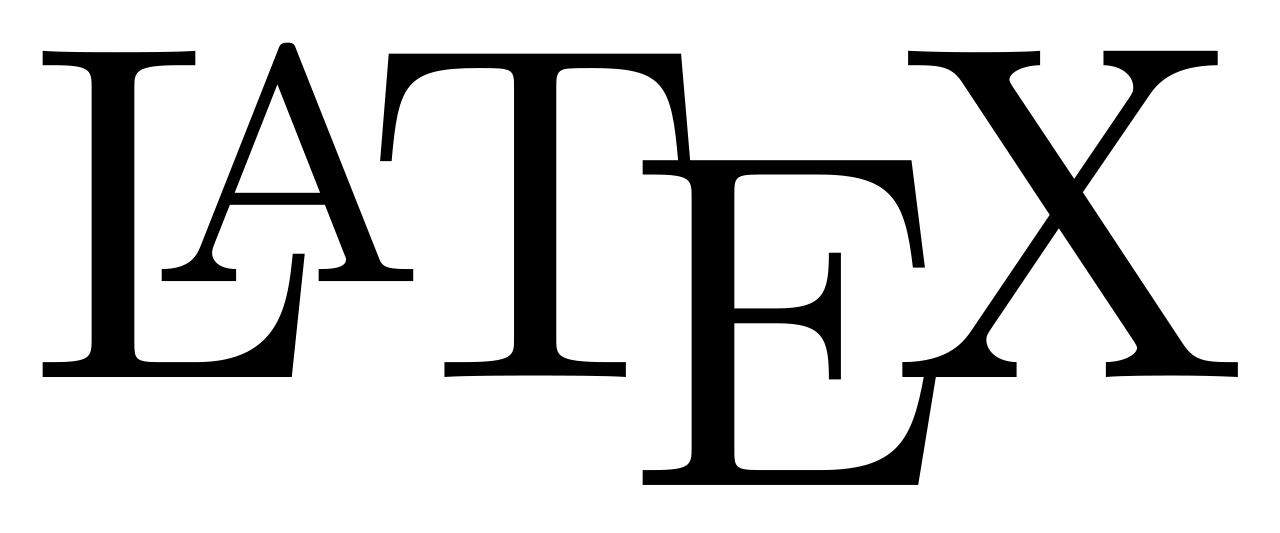
\includegraphics[width=\linewidth]{figs/1280px-LaTeX-logo.png}
		\source{Wikimedia Commons \cite{wikimedia-latex}.}
	\end{minipage}
\end{figure}

Além de figuras, \index{figuras} é possível inserir caixas de texto de diversos tipos, como axiomas, teoremas etc. Elas podem ser configuradas e novos tipos delas podem ser criados no arquivo \begin{verbatim}config/envs.tex\end{verbatim}.

Existem pacotes que permitem criar figuras e gráficos no próprio código \LaTeX. Por exemplo, temos

\begin{itemize}
    \item PGFPlots \url{http://pgfplots.sourceforge.net/}
    \item TikZ \url{http://www.texample.net/tikz/examples/all/}
    \item Metapost \url{http://tex.loria.fr/prod-graph/zoonekynd/metapost/metapost.html}
    \item PSTricks \url{https://tug.org/PSTricks/main.cgi?file=examples}
\end{itemize}

\begin{question}
    Explique como Isaac Newton usaria cada um dos pacotes seguintes, se vivesse no tempo presente:
    \begin{enumerate}[label=(\Alph*)]
        \item Metapost
        \item TikZ
        \item PGFPlots
        \item PSTricks
    \end{enumerate}
\end{question}

\begin{solution}
    \begin{enumerate}[label=(\Alph*)]
        \item Para fazer figuras 3D.
        \item Para fazer diagramas.
        \item Para traçar gráficos.
        \item Para fazer de um tudo.
    \end{enumerate}
\end{solution}

\section{Soluções deste capítulo}

\printsolutions
%\clearpage
%%\fancyfoot[CO,CE]{}
\fancyfoot[LO]{\small}
\fancyfoot[RO]{\small}
%\fancyfoot[CE]{\Author}
\fancyfoot[LE]{\small}
\fancyfoot[RE]{\small}

\begin{discussion}

\hfill

\begin{center}
  \textsc{\large Criando quadros}\\
\end{center}

\vspace{1ex}

\begin{flushright}
  \textbf{Leonardo Luiz e Castro} \\
  \vspace{1ex}
  \textit{\small Instituto de Física} \\
  \textit{\small Universidade de Brasília} \\
\end{flushright}

\addcontentsline{toc}{section}{Texto complementar -   Criando quadros (Leonardo Luiz e Castro)}

\vspace{1ex}

\section*{O que são quadros?}

Quadros são parecidos com tabelas, com a diferença de que não contêm dados numéricos, mas sim informação textual. Aparentemente, a ABNT é pioneira no mundo em se preocupar com tal distinção.

\section*{Exemplo de quadro em \LaTeX?}

Preferi listar os quadros como figuras. Vi algum livro que fazia assim... Veja como a figura \ref{fig:estados-da-materia} ficou interessante! Lembre-se que só é possível inserir uma figura dentro de um ambiente como este se a opção de não flutuação ([H]) for utilizada.

\begin{figure}[H]
	\centering
	\begin{minipage}{\hsize}
		\centering
		\taburulecolor{white}\arrayrulecolor{white}
		\caption{Quadro de caracterização dos estados da matéria.}
		\label{fig:estados-da-materia}
		\begin{tabular}{| >{\centering\cellcolor{verde_UnB}\color{white}}p{0.11\hsize} | >{\centering\cellcolor{verde_UnB}\color{white}}p{0.12\hsize} | >{\centering\cellcolor{verde_UnB}\color{white}}p{0.12\hsize} | >{\centering\cellcolor{verde_UnB}\color{white}\footnotesize}p{0.11\hsize} | >{\centering\cellcolor{verde_UnB}\color{white}\footnotesize}p{0.16\hsize} | >{\centering\cellcolor{verde_UnB}\color{white}\footnotesize}p{0.17\hsize} |}
			\hline
			{\bf Estado} & {\bf Volume} & {\bf Forma} & {\bf É fluido?} & {\bf É matéria condensada?} & {\bf É compressível?} \tabularnewline
			\hline
		\end{tabular}
		\begin{tabular}{| >{\centering\cellcolor{verde_UnB!70}\color{white}\small}p{0.11\hsize} | >{\centering\cellcolor{verde_UnB!50}\color{black}\small}p{0.12\hsize} | >{\centering\cellcolor{verde_UnB!50}\color{black}\small}p{0.12\hsize} | >{\centering\cellcolor{verde_UnB!50}\color{black}\small}p{0.11\hsize} | >{\centering\cellcolor{verde_UnB!50}\color{black}\small}p{0.16\hsize} | >{\centering\cellcolor{verde_UnB!50}\color{black}\small}p{0.17\hsize} |}
			\hline
			Gasoso & ajustável & ajustável & sim & não & muito \tabularnewline
			\hline
			Líquido & fixo & ajustável & sim & sim & pouco \tabularnewline
			\hline
			Sólido & fixo & fixa & não & sim & não \tabularnewline
			\hline
		\end{tabular}
		\source{elaboração do autores de Física para Ciências Agrárias e Ambientais (Leonardo Castro e Olavo Filho).}
	\end{minipage}
\end{figure}

\end{discussion}

%\cleardoublepage

%\chapter{Ambientes}

\thispagestyle{empty}

Este modelo disponibiliza alguns ``ambientes'', ou seja, caixas de texto com formatação especial para certos tipos de elementos que são automaticamente numerados (e.g. teorema 1.1, teorema 1.2 etc.). Ambientes podem ser criados e configurados por edição do arquivo envs.tex da pasta config.

\section{Exemplos de ambientes disponíveis}

\begin{axiom}
    \LaTeX produz equações mais bonitas que qualquer editor WYSIWYG.
\end{axiom}

\begin{theorem}\textsc{teorema LaTeX-WYSIWYG}
    Todo físico prefere usar código \LaTeX puro que qualquer editor WYSIWYG.
\end{theorem}

\index{\LaTeX} % entrada para o índice remissivo
\index{WYSIWYG}

\begin{demonstration}
    Físicos gostam de equações bonitas. Editores What-You-See-Is-What-You-Get não são apropriados para fazer equações bonitas.\footnote{É certo que há editores WYSIWYG baseados em \LaTeX, mas eles não nos dão o mesmo nível de controle.} Logo, se algum físico preferisse usar um editor WYSIWYG no lugar de \LaTeX, não seria muito inteligente. Como todo físico é inteligente, o teorema está demonstrado \textit{ad absurdum}.
\end{demonstration}

\begin{example}
    Einstein usaria um editor WYSIWYG ou \LaTeX? \\
    Einstein era físico. Portanto, usando o teorema LaTeX-WYSIWYG, concluímos que ele usaria \LaTeX.
\end{example}

\begin{question}
    Einstein usaria um editor WYSIWYG ou \LaTeX?
\end{question}

\begin{solution}
    Einstein era físico. Portanto, usando o teorema LaTeX-WYSIWYG, concluímos que ele usaria \LaTeX.
\end{solution}

\begin{question}
    Marie Curie usaria um editor WYSIWYG ou \LaTeX?
\end{question}

\begin{solution}
    Deixamos esta sem resposta para o estudante se esforçar mais.
\end{solution}

\clearpage

\section{Soluções deste capítulo}

\printsolutions
%\cleardoublepage

%\chapter{Conclusão}

\thispagestyle{empty}

Você deve começar a editar o seu livro agora mesmo!
%\cleardoublepage


\chapter{Errores}

Holaaaa


% Apêndices:

\renewcommand\appendixname{ANEXOS}
\renewcommand\appendixpagename{ANEXOS}
\renewcommand{\appendixtocname}{ANEXOS}

\begin{appendices}

% Formatando como em "APÊNDICE A -- Título do apêndice":
% Ref.: https://tex.stackexchange.com/a/479364/91816

\makeatletter
\def\@chapter[#1]#2{\ifnum \c@secnumdepth >\m@ne
    \refstepcounter{chapter}%
    \typeout{\thechapter.}%
    \addcontentsline{toc}{chapter}%
    {\thechapter\space\textendash\space\ #1}% <-- modification
  \else
    \addcontentsline{toc}{chapter}{#1}%
  \fi
  \chaptermark{#1}%
  \addtocontents{lof}{\protect\addvspace{10\p@}}%
  \addtocontents{lot}{\protect\addvspace{10\p@}}%
  \if@twocolumn
    \@topnewpage[\@makechapterhead{#2}]%
  \else
    \@makechapterhead{#2}%
    \@afterheading
  \fi}
\makeatother

% Reiniciando contador de capítulo e seção:

\setcounter{chapter}{0}
\setcounter{section}{0}

%\chapter{Referencias}

\thispagestyle{empty} 

Este modelo usa BibTeX para configurar as referências. O arquivo main.bib contém várias entradas de bibliografia como modelos \cite{article,book,booklet,inbook}. Esses modelos podem ser utilizados para incluir outras entradas e citá-las por meio do seguinte comando:
\begin{verbatim}
\cite{nome_da_entrada}
\end{verbatim}

Por exemplo , a entrada
\verbatimfont{\small}
\begin{verbatim}
@article{greenwade93,
    author  = "George D. Greenwade",
    title   = "The {C}omprehensive {T}ex {A}rchive {N}etwork ({CTAN})",
    year    = "1993",
    journal = "TUGBoat",
    volume  = "14",
    number  = "3",
    pages   = "342--351"
}
\end{verbatim}
\verbatimfont{\normalfont}
pode ser citada no texto com
\begin{verbatim}
\cite{greenwade93}
\end{verbatim}
e a citação apareceria assim: \cite{greenwade93}.

Para fazer uma citação direta no formato ABNT, criamos o ambiente \verb|citacao|, que é uma simples generalização do ambiente \verb|quotation| (habilitado por padrão) com um campo específico de autor. Veja o exemplo a seguir:
\begin{verbatim}
\begin{citacao}{Carl Sagan}
    Alegações extraordinárias exigem evidências extraordinárias.
\end{citacao}
\end{verbatim}
Esse código gera uma citação assim:
\begin{citacao}{Carl Sagan}
    Alegações extraordinárias exigem evidências extraordinárias.
\end{citacao}
O comando \verb|\cite{...}| pode ser usado como indicação do autor:
\begin{verbatim}
\begin{citacao}{\cite{greenwade93}}
TEX is a typesetting program designed for high-quality composition of material that contains a lot of mathematical and technical expressions. It has been adopted by many authors and publishers who generate technical books and papers. It was created by Professor Donald E. Knuth of Stanford University, originally for preparation of his book series ``The Art of Computer Programming''. TEX has been made freely available by Knuth.
\end{citacao}
\end{verbatim}
Naturalmente, a referência \verb|grennwade93| deve estar definida no arquivo BibTeX (aqui, \verb|main.bib|). Confira o resultado:
\begin{citacao}{\cite{greenwade93}}
TEX is a typesetting program designed for high-quality composition of material that contains a lot of mathematical and technical expressions. It has been adopted by many authors and publishers who generate technical books and papers. It was created by Professor Donald E. Knuth of Stanford University, originally for preparation of his book series ``The Art of Computer Programming''. TEX has been made freely available by Knuth.
\end{citacao}



%\cleardoublepage

%\chapter{Tabelas}

\thispagestyle{empty} 

A tabela \ref{tab:SI-basicas} mostra algumas unidades básicas do SI.

\begin{table}
\begin{minipage}{\hsize}
\begin{center}
	\caption{Algumas unidades básicas do SI.}
	\label{tab:SI-basicas}
	\begin{tabular}{P{0.40\hsize}|P{0.5\hsize}}
		\hline
		\textbf{Grandeza} & \textbf{Unidade} \\
		\hline
		comprimento & metro (\si{\meter}) \\
		\hline
		massa & quilograma (\si{\kilo\gram}) \\
		\hline
		tempo & segundo (\si{\second}) \\
		\hline
		corrente elétrica & ampère (\si{\ampere}) \\
		\hline
		temperatura & kelvin (\si{\kelvin}) \\
		\hline
		quantidade de matéria & mol (\si{\mol}) \\
		\hline
		intensidade luminosa & candela (\si{\candela}) \\
		\hline
	\end{tabular}
	\source{adaptado do livro Física para Ciências Agrárias e Ambientais, de Leonardo Luiz e Castro e Olavo Leopoldino da Silva Filho.}
\end{center}
\end{minipage}
\end{table}


É uma boa ideia usar o pacote ``longtable'' para criar tabelas, \index{tabelas} pois assim uma mesma tabela pode ocupar várias páginas. Dê uma olhada no código da lista de símbolos, pois ela foi feita com esse pacote.

%\cleardoublepage

\end{appendices}

% Anexos:


\renewcommand\appendixname{ANEXO}
\renewcommand\appendixpagename{ANEXOS}
\renewcommand{\appendixtocname}{ANEXOS}

\begin{appendices}

% Formatando como em "APÊNDICE A -- Título do apêndice":
% Ref.: https://tex.stackexchange.com/a/479364/91816

\makeatletter
\def\@chapter[#1]#2{\ifnum \c@secnumdepth >\m@ne
    \refstepcounter{chapter}%
    \typeout{\thechapter.}%
    \addcontentsline{toc}{chapter}%
    {\thechapter\space\textendash\space\ #1}% <-- modification
  \else
    \addcontentsline{toc}{chapter}{#1}%
  \fi
  \chaptermark{#1}%
  \addtocontents{lof}{\protect\addvspace{10\p@}}%
  \addtocontents{lot}{\protect\addvspace{10\p@}}%
  \if@twocolumn
    \@topnewpage[\@makechapterhead{#2}]%
  \else
    \@makechapterhead{#2}%
    \@afterheading
  \fi}
\makeatother

% Reiniciando contador de capítulo e seção:

\setcounter{chapter}{0}
\setcounter{section}{0}

%\chapter{Figuras de exemplo}

\thispagestyle{empty} 

% Fonte: https://tex.stackexchange.com/a/231741/91816 (Gonzalo Medina)

\noindent\includegraphics[width=3cm]{example-image-a}\qquad
\includegraphics[width=3cm]{example-image-golden}\qquad
\includegraphics[width=3cm]{example-grid-100x100pt}

\noindent\includegraphics[height=5cm]{example-image-b} 

\noindent\includegraphics[scale=0.5]{example-image-c} 

\noindent\includegraphics[width=3cm]{example-image} 
%\cleardoublepage

%\chapter{Logo LaTeX}

\thispagestyle{empty} 

\vfill

\begin{center}
{\fontsize{50pt}{800pt}\selectfont \LaTeX}\
\end{center}

\vfill

\begin{center}
{\color{cinza_UnB}\fontsize{50pt}{800pt}\selectfont \LaTeX}\
\end{center}

\vfill

\begin{center}
{\color{verde_UnB}\fontsize{50pt}{800pt}\selectfont \LaTeX}\
\end{center}

\vfill
%\cleardoublepage

\end{appendices}
-
% Parte Pós-Textual:
\backmatter

% Referências (Bibliografia):

\singlespacing

\bibliographystyle{abntex2-alf}
\bibliography{main}
\cleardoublepage

% Índice Remissivo, controlado pelo comando \index{...} em meio ao texto:

\phantomsection
\printindex

\end{document}
